\begin{figure}
	\centering
	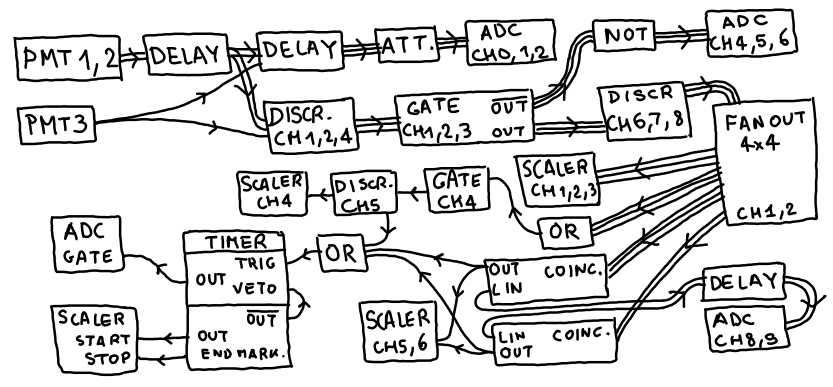
\includegraphics[width=0.9\textwidth]{immagini/circuitone} \\
	\vspace{1em}
	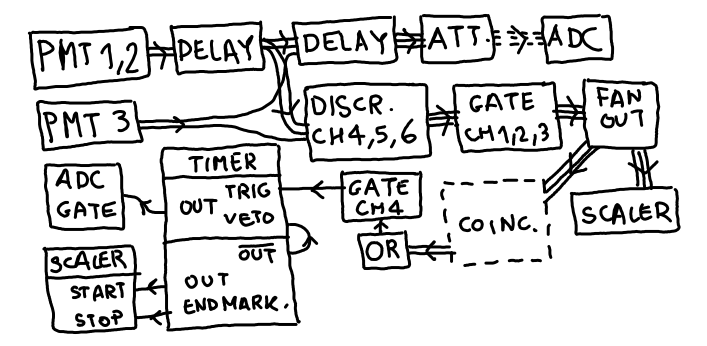
\includegraphics[width=0.6\textwidth]{immagini/circuitob}
	\caption{Circuito dell'apparato A (sopra) e dell'apparato B (sotto).}
	\label{circuitone}
\end{figure}

\subsection{Circuito A}

\subsubsection{Descrizione del circuito}

Il primo circuito assemblato è rappresentato in \autoref{circuitone} in alto.

Le uscite dei PMT sono inviate ai discriminatori, le cui uscite attraversano un modulo di antiretrigger (tempo morto di \SI{1}{\micro s}) e vengono usate per costruire funzioni logiche. I segnali dei PMT vengono anche inviati all'ADC attraverso un attenuatore per regolare il fondoscala.

Per quanto riguarda la parte logica, costruiamo e mettiamo in tempo tre tipi di trigger:
\begin{itemize}
	\item PMT singolo;
	\item coincidenza a 2;
	\item coincidenza a 3.
\end{itemize}
% Il trigger di canale è semplicemente il segnale discriminato del PMT corrispondente; quello di coincidenze è dato dall'uscita di lunga durata del modulo stesso. Mandiamo questi segnali all'ADC in modo che il trigger di canale arrivi in contemporanea con il segnale analogico del canale stesso. Se in quel momento c'è anche un trigger di coincidenza, sappiamo se l'evento ci è arrivato da una coincidenza anziché da un canale singolo. Abbiamo fatto tutto questo per acquisire tutti i canali contemporaneamente ed agevolare la lettura dei dati via software. Purtroppo il \emph{crosstalk}%
% \footnote{Spiegheremo come ci siamo accorti di questo problema nella \autoref{ref}.} presente nell'ADC ha afflitto pesantemente le misure fatte con questo circuito.
Ogni segnale logico viene mandato sia al contatore che a un canale dell'ADC
per salvare e poter leggere via software i trigger.

% Per dare precedenza agli eventi più rari abbiamo collegato questi trigger ad un modulo \emph{or} ritardando i trigger singoli rispetto a quelli di coincidenze a 2 e questi ultimi rispetto alle coincidenze a 3. L'uscita dell'\emph{or} era poi inviata ad un \emph{timer} che generava il gate dell'ADC. L'altro canale di questo \emph{timer} veniva usato per avviare o fermare le acquisizioni.

Poiché i trigger sui singoli rivelatori hanno un rate molto più alto delle coincidenze
abbiamo introdotto una decimazione con un tempo morto regolabile.

\subsubsection{Problemi riscontrati}

Purtroppo il circuito presentava dei problemi.

\paragraph{Bit stuck}

Il più evidente fin da subito è stato il \emph{bit stuck}: il terzo bit meno significativo dei dati in formato binario è sempre 1.
Gli istogrammi presentano delle lacune di \SI{4}{digit} ogni \SI{4}{digit}. Risolviamo questo problema usando bin del tipo $[0,8)+n$ con  $n=0,1,2,\dots$ nei vari istogrammi.

\paragraph{Temporizzazione dei trigger}

% Poi abbiamo visto che i segnali in coincidenza mostravano un'energia minore di quelli non in coincidenza quando usavamo il modulo \emph{or}.
% Tale differenza era data da un'errata temporizzazione dei segnali.
% Uno dei motivi per cui abbiamo usato l'or all'interno del circuito era il poter calibrare l'acquisizione durante le misure di lunga durata alternando il segnale del PMT singolo a quello delle coincidenze.
% Per fare questo abbiamo posto un tempo morto sul trigger degli eventi non in coincidenza, ma il modulo che abbiamo usato per farlo ha un jitter significativo se gli impulsi che genera sono più lunghi di \SI{1}{ms}. Di conseguenza abbiamo segnali non più in tempo con il gate dell'ADC e l'energia misurata non è quella effettiva.
% Non avendo più motivi per usarlo, abbiamo rimosso l'or dal circuito.
%
Poiché l'ADC misura la carica del segnale in un certo intervallo temporale dato da un segnale di gate
che viene avviato dai trigger,
se due trigger non hanno lo stesso ritardo rispetto al segnale del rivelatore
la calibrazione delle letture dell'ADC è diversa per i due trigger.
Nel nostro circuito le coincidenze sono fatte con moduli uguali che ricevono lo stesso input
e hanno ritardi brevi e stabili,
mentre i trigger sui singoli rivelatori seguono una catena elettronica diversa;
in particolare il modulo che introduce il tempo morto per la decimazione ha un jitter significativo.
Abbiamo effettivamente osservato la diversa calibrazione dell'ADC a seconda del trigger,
e poiché i trigger sui singoli rivelatori erano proprio a scopo di calibrazione, abbiamo rinunciato a usarli.

\paragraph{Dipendenza della calibrazione dal rate}

Confrontando gli spettri del \na{} abbiamo visto che i fotoni emessi dalla sorgente con attività maggiore avevano energia maggiore.
Il grafico in \autoref{distanze} mostra l'energia dei fotopicchi del sodio in funzione del rate misurato ponendo la sorgente ad attività elevata a varie distanze dal rivelatore.
I dati della misura si trovano \autoref{tabella forte}.

\marginpar{Nella \autoref{distanze}
la sorgente debole non deve essere una riga
ma un punto perché ha un rate.}

\begin{figure}[h]
\centering
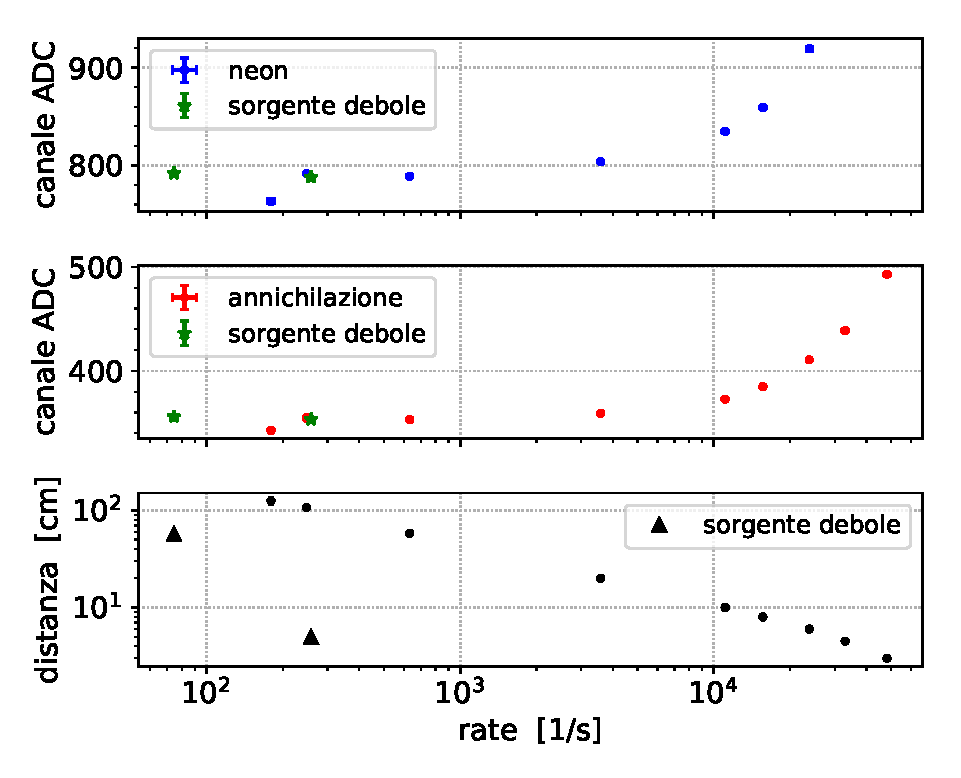
\includegraphics[width=28 em]{immagini/naforte}
\caption{Posizione dei fotopicchi del sodio in funzione del rate di eventi ponendo la sorgente a diverse distanze dal rivelatore. In alcune delle acquisizioni non era visibile il picco del neon oppure era talmente deformato da rendere privo di senso il fit gaussiano. La linea tratteggiata mostra la posizione dello stesso picco usando la sorgente di attività minore.}
\label{distanze}
\end{figure}

\begin{table}[h]
\centering
\begin{tabular}{c|c|c}
rate [1/s] & Beta [digit] & Neon [digit] \\
\hline
 179.5$\,\pm\,$0.2 & 342.86$\,\pm\,$0.52 & 763.4$\,\pm\,$2.4 \\
 247.7$\,\pm\,$0.2 & 354.76$\,\pm\,$0.45 & 791.7$\,\pm\,$1.3 \\
 632.8$\,\pm\,$0.2 & 353.26$\,\pm\,$0.35 & 788.8$\,\pm\,$1.4 \\
3583.7$\,\pm\,$0.7 & 359.26$\,\pm\,$0.39 & 803.7$\,\pm\,$1.1 \\
  11086$\,\pm\,$14 & 372.79$\,\pm\,$0.24 & 834.8$\,\pm\,$1.0 \\
  15613$\,\pm\,$15 & 384.92$\,\pm\,$0.27 & 859.16$\,\pm\,$0.97 \\
  23784$\,\pm\,$24 & 410.76$\,\pm\,$0.45 & 919.4$\,\pm\,$2.5 \\
  32948$\,\pm\,$27 & 438.8$\,\pm\,$1.2 &         \\
  48190$\,\pm\,$24 & 492.90$\,\pm\,$0.76 &        
\end{tabular}

\caption{Tabella dei dati in \autoref{distanze}. ``Beta'' indica la media del picco di annichilazione, ``Neon'' quella del relativo fotopicco.}
\label{tabella forte}
\end{table}

Pensiamo che tale effetto sia dovuto ad un pile-up nella digitalizzazione in quanto l'ADC ha un tempo di conversione di \SI{60}{\micro s}.
\marginpar{Dalle misure fatte l'ultimo giorno sappiamo che
il problema non può essere solo il pile-up della digitalizzazione.
Inoltre avevamo anche escluso che il problema fosse solo il pile-up dei segnali.}
Dal grafico si evince che anche con un rate di eventi minore di \SI{10}{ms^{-1}} il problema persiste perché la distribuzione temporale tra un evento e il successivo non è uniforme, ma esponenziale. Quindi tra due eventi consecutivi intercorre spesso un piccolo intervallo di tempo.
Abbiamo quindi deciso di utilizzare la sorgente ad attività minore per misurare la massa dell'elettrone e quella ad attività maggiore per le misure in cui non ci interessa l'energia degli eventi o cerchiamo eventi rari.